%% LyX 2.3.5.2 created this file.  For more info, see http://www.lyx.org/.
%% Do not edit unless you really know what you are doing.
\documentclass[british]{beamer}
\usepackage[latin9]{inputenc}
\usepackage{babel}
\usepackage{algorithm2e}
\usepackage{amssymb}
\usepackage{graphicx}
\ifx\hypersetup\undefined
  \AtBeginDocument{%
    \hypersetup{unicode=true}
  }
\else
  \hypersetup{unicode=true}
\fi

\makeatletter
%%%%%%%%%%%%%%%%%%%%%%%%%%%%%% Textclass specific LaTeX commands.
% this default might be overridden by plain title style
\newcommand\makebeamertitle{\frame{\maketitle}}%
% (ERT) argument for the TOC
\AtBeginDocument{%
  \let\origtableofcontents=\tableofcontents
  \def\tableofcontents{\@ifnextchar[{\origtableofcontents}{\gobbletableofcontents}}
  \def\gobbletableofcontents#1{\origtableofcontents}
}

%%%%%%%%%%%%%%%%%%%%%%%%%%%%%% User specified LaTeX commands.
\DeclareMathAlphabet{\mathcal}{OMS}{cmsy}{m}{n}
\usetheme[oldstylearrows,nologo,numbers,algorists]{CIMAT}

% or ...

\setbeamercovered{transparent}
% or whatever (possibly just delete it)
\usepackage[euler-digits]{eulervm}
\usefonttheme{professionalfonts}
\usepackage{dsfont}
%\usepackage[table]{xcolor}
%\usepackage{booktabs}

%\usepackage[usenames,dvipsnames]{xcolor}
\usepackage{tcolorbox}
\usepackage{tabularx}
\usepackage{array}
\usepackage{colortbl}
\tcbuselibrary{skins,fitting}

\newcolumntype{Y}{>{\raggedleft\arraybackslash}X}

\DeclareMathOperator{\posdef}{+def}
\DeclareMathOperator{\tr}{tr}
\DeclareMathOperator{\cov}{cov}
\DeclareMathOperator{\variance}{var}
\DeclareMathOperator{\lcp}{lcp}
\renewcommand{\mathbf}{\boldsymbol}
\DeclareMathOperator{\idv}{div}
\DeclareMathOperator{\diag}{diag}

\SetKwInOut{Input}{Input}
\SetKwInOut{Output}{Output}
\SetKwInOut{Data}{Parameters}
\SetKwInOut{Result}{output}
\SetKw{struct}{struct}
\SetKw{KwTo}{to}
\SetKw{Throw}{throw}
\SetKw{KwRet}{return}
\SetKw{Return}{return}
\SetKwProg{Function}{function}{:}{end}
\SetKwProg{lFunction}{function}{}{}
\SetKwBlock{Begin}{begin}{end}
\SetKwRepeat{Repeat}{repeat}{until}
\SetKwIF{If}{ElseIf}{Else}{if}{then}{else if}{else:}{end}
\SetKwSwitch{Switch}{Case}{Other}{select}{for}{case}{otherwise}{end}{end}
\usepackage{algpseudocode}
\SetKwFor{For}{for}{do:}{end}
\SetKwFor{ForPar}{parallel for}{do:}{end}
\SetKwFor{ForEach}{for each}{do:}{end}
\SetKwFor{ForAll}{for all}{do:}{end}
\SetKwFor{While}{while}{do:}{end}

\SetKw{Static}{static}
\SetKw{Const}{const}
\SetKw{Struct}{struct}
\SetKw{Class}{class}
\SetKw{New}{new}
\SetKw{Delete}{delete}
\SetKw{Char}{char}
\SetKw{Integer}{int}
\SetKw{Long}{long}
\SetKw{Unsigned}{unsigned}
\SetKw{Signed}{signed}
\SetKw{Boolean}{bool}
\SetKw{KwNot}{not}
\SetKw{KwAnd}{and}
\SetKw{KwOr}{or}
\SetKw{KwXor}{xor}

\SetKwFunction{node}{node}
\SetKwFunction{sort}{std::sort}
\SetKwFunction{lcp}{lcp}
\SetKwFunction{strlen}{strlen}
\SetKwFunction{strcmp}{strcmp}
\SetKwFunction{fibonacci}{fibonacci}
\SetKwFunction{pushback}{push-back}
\SetKwFunction{alphanumeric}{to-alpha}
\SetKwFunction{back}{back}
\SetKwFunction{neighborhood}{neighborhood}
\SetKwFunction{buildsuffix}{build-suffix-array}
\SetKwFunction{isEmpty}{is-empty}
\SetKwFunction{isNull}{is-null}
\SetKwFunction{isBetter}{can-improve}
\SetKwFunction{isUnvisited}{is-unvisited}
\SetKwFunction{isValid}{is-valid}
\SetKwFunction{improve}{visit-or-improve}
\SetKwFunction{mycomparator}{cmp}

\SetKwFunction{memset}{std::memset}
\SetKwFunction{sizeof}{sizeof}
\SetKwFunction{map}{std::map}
\SetKwFunction{addword}{add-word}
\SetKwFunction{findword}{find-word}
\SetKwFunction{isEmpty}{is-empty}
\SetKwFunction{isNull}{is-null}

\SetSideCommentRight

\newcolumntype{Y}{>{\raggedleft\arraybackslash}X}

\tcbset{smallvalues/.style={enhanced,fonttitle=\bfseries,fontupper=\normalsize\sffamily,
colback=zorange!10!white,colframe=zorange!90!black,colbacktitle=zorange!90!white,
coltitle=white,center title}}

\makeatother

\usepackage{listings}
\renewcommand{\lstlistingname}{Listing}

\begin{document}
\title[Dynamic Programming]{Dynamic Programming}
\author[Ulises Tirado Zatarain]{Ulises Tirado Zatarain~  \inst{1}\\
(ulises.tirado@cimat.mx) }
\institute[Algorists]{\inst{1}Algorists Group}
\date[Nov, 2020]{November, 2020}

\makebeamertitle
\pgfdeclareimage[height=0.75cm]{algorists}{algorists.png}
\logo{\pgfuseimage{algorists}}

\AtBeginSubsection[]{
  \frame<beamer>{ 
    \frametitle{Outline}   
    \tableofcontents[currentsection,currentsubsection] 
  }
}

%\beamerdefaultoverlayspecification{<+->}
\begin{frame}{Outline}

\tableofcontents{}

\end{frame}

\section{Introduction}

\subsection[Definitions]{Definitions}
\begin{frame}{What is dynamic programming?}

\begin{definition}[Dynamic Programming]
 It's a technique for mathematical programming (optimization), or
in other words, a paradigm to problem solving. So, the word ``programming''
is not directly meaning a computer program or an algorithm. The actual
meaning is more similar to linear programming or planning or taking
decisions.
\end{definition}

\begin{itemize}
\item It consists in:

\begin{itemize}
\item Split the problem in smaller sub-problems:
\begin{itemize}
\item recurrence relationship
\item optimal sub-structure
\end{itemize}
\item We stop when have a trivial problems (base cases)
\item Store smaller solutions (memoization, states) 
\item Merge the solutions when is need it
\item Difference with D\&C: \textbf{overlapping and compute a value}
\end{itemize}
\end{itemize}
\end{frame}


\subsection{A particular problem}
\begin{frame}{Recurrence relationship}

Fibonacci sequence ($0,1,1,2,3,5,\ldots$) is the simplest examples

\begin{center}
$F_{N}=\begin{cases}
N & N\in\{0,1\}\\
F_{N-1}+F_{N-2} & N>1
\end{cases}$
\par\end{center}
\begin{block}{Fibonacci numbers}
Given $Q$ queries compute the $N$-th Fibonacci number for each
of them. Each query is a single line with a single integer $N$. Your
task is write a function which receives the integer $N$ as input
and should return the $N$-th Fibonacci number.
\end{block}
\end{frame}


\subsection{Naive solutions and limitations}
\begin{frame}{Fibonacci classic iterative implementation}

\begin{algorithm}[H]
\Const \Integer $MAX = 90$\;
\Function{\Long \Integer \fibonacci{\Integer $N$}}{
	\lIf{$n < 0$ \KwOr $N > MAX$}{\Throw "Out of range."}
	\Long $current=0$, $next=1$\;
	\For{$k=1$ \KwTo $N$}{
		\Long $aux=current+next$\;
		$current=next$\;
		$next=aux$\;
	}
	\Return{$current$}\;
}
\end{algorithm}
\end{frame}

\begin{frame}{Fibonacci classic recursive implementation}

\begin{algorithm}[H]
\Const \Integer $MAX = 90$\;
\Function{\Long \Integer \fibonacci{\Integer $N$}}{
	\lIf{$N < 0$ \KwOr $N > MAX$}{\Throw "Out of range."}
	\lIf{$N < 2$}{\Return{$N$}}
	\Return{\fibonacci{$N-1$} $+$ \fibonacci{$N-2$}}\;
}
\end{algorithm}
\end{frame}

\begin{frame}{Problems with the classic implementations}

\begin{itemize}
\item \visible<1->{In the iterative implementation we compute all the values
for every query.}
\item \visible<2->{In the recursive one, some values are computed twice
(or more times), in particular for $F(4)$:
\end{itemize}
\begin{center}
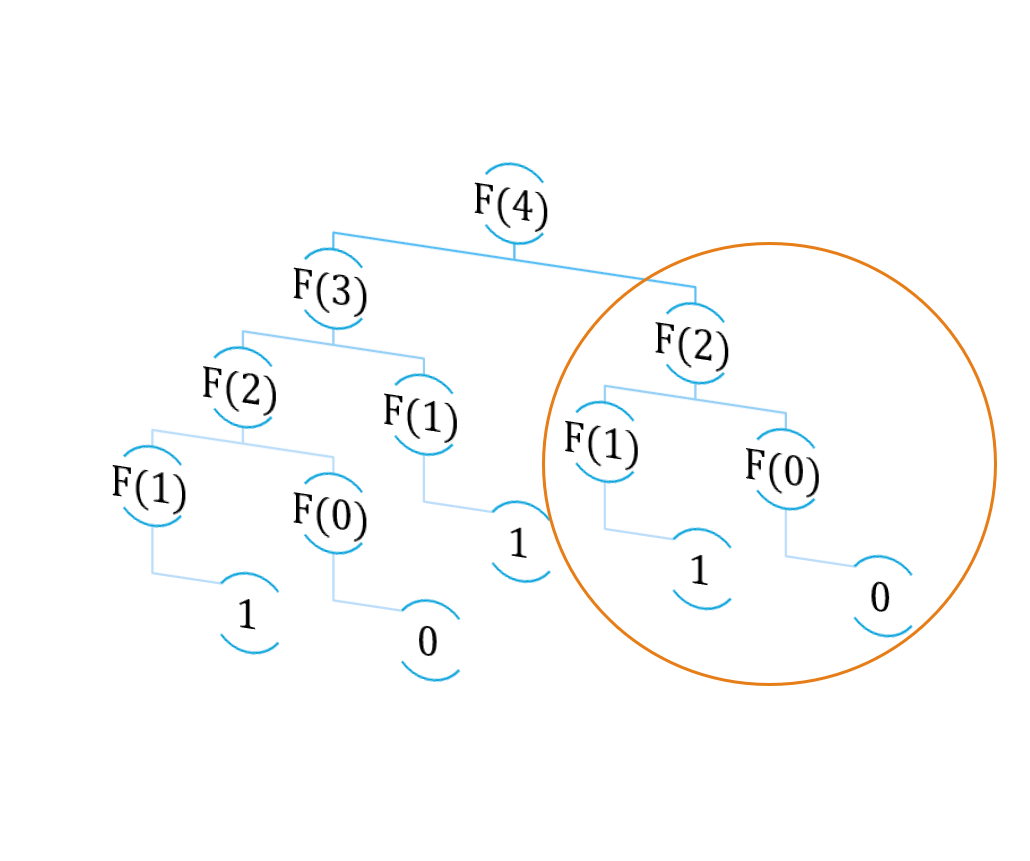
\includegraphics[viewport=47.9612bp 81.5447bp 479.612bp 340.569bp,clip,scale=0.5]{figures/fibonacci-tree-redundance}}
\par\end{center}
\begin{itemize}
\item \visible<3->{This is called \textbf{overlapping}}
\end{itemize}
\end{frame}

\begin{frame}{Complexity?}
\begin{itemize}
\item \visible<1->{What is run time complexity for the iterative function?
} \visible<2->{$O(N)$}
\item \visible<3->{What is run time complexity for the recursive one? } \visible<4->{$O(2^{N})$}
\item \visible<5->{What is the run time complexity for the whole program?}
\begin{itemize}
\item \visible<6->{Iterative: $O(QN)$}
\item \visible<7->{Recursive: $O(2^{N}Q)$}
\end{itemize}
\item \visible<8->{What about the memory?}
\begin{itemize}
\item \visible<9->{Iterative: $O(1)$}
\item \visible<10->{Recursive: $O(N)$--Why?} \visible<11->{Stack}
\end{itemize}
\end{itemize}
\end{frame}


\section{Algorithm design}

\subsection{Design}
\begin{frame}{Design and implementations}

There are two ways to implement dynamic programming:
\begin{itemize}
\item Bottom-up (iterative implementation)
\begin{itemize}
\item Solve \textbf{all the the possible smaller problems} before the bigger
one
\end{itemize}
\item Top-down (recursive implementation)
\begin{itemize}
\item Solve \textbf{only the instances which are actually needed} for a
given problem
\end{itemize}
\item Both solve the problem in efficient way, the discussion may end up
in \emph{religious} arguments.
\end{itemize}
\end{frame}

\begin{frame}{Fibonacci bottom-up implementation}
Solve all the the possible smaller problems before the bigger one:
\begin{algorithm}[H]
\Const \Integer $MAX = 90$\;
\Const \Long \Integer $UNDEFINED = -1$\;
\Long \Integer $memo[MAX + 1]$\;
\memset{$memo$, $UNDEFINED$, \sizeof{$memo$}}\;
$memo[0]=0$; $memo[1]=1$\;
\Function{\Long \Integer \fibonacci{\Integer $N$}}{
	\lIf{$n < 0$ \KwOr $N > MAX$}{\Throw "Out of range."}
	\If{$memo[N]==UNDEFINED$}{
		\For{$k=2$ \KwTo $N$}{
			$memo[k]=memo[k-1]+memo[k-2]$\;
		}
	}
	\Return{$memo[N]$}\;
}
\end{algorithm}
\end{frame}

\begin{frame}{Fibonacci top-down implementation}

Solve only the instances which are actually needed for a given problem:

\begin{algorithm}[H]
\Const \Integer $MAX = 90$\;
\Const \Long \Integer $UNDEFINED = -1$\;
\Long \Integer $memo[MAX + 1]$\;
\memset{$memo$, $UNDEFINED$, \sizeof{$memo$}}\;
$memo[0]=0$; $memo[1]=1$\;
\Function{\Long \Integer \fibonacci{\Integer $N$}}{
	\lIf{$N < 0$ \KwOr $N > MAX$}{\Throw "Out of range."}
	\lIf{$memo[N] \neq UNDEFINED$}{\Return{$memo[N]$}}
	$memo[n]=$ \fibonacci{$N-1$} $+$ \fibonacci{$N-2$}\;
	\Return{$memo[N]$}\;
}
\end{algorithm}
\end{frame}


\subsection{Analysis}
\begin{frame}{Complexity analysis}
\begin{itemize}
\item \visible<1->{What is the run time complexity in both cases?} \visible<2->{$O(\max(Q,N))$}
\item \visible<3->{And the memory complexity?} \visible<4->{$O(N)$}
\item \visible<5->{Generally speaking, DP solutions have a run time complexity
$O(M\times S)$ and in memory $O(M)$; where $M$ is the number of
sub-problems problem and $S$ is the complexity of solving each sub-problem.}
\end{itemize}
\end{frame}

\section{More problems}

\subsection{Unidimensional problems}
\begin{frame}{Coin change (brainstorming/coding)}
\begin{block}{Coin change (\href{https://leetcode.com/problems/coin-change/}{source: LeetCode})}
You are given coins of different denominations and a total amount
of money amount. Write a function to compute the fewest number of
coins that you need to make up that amount. If that amount of money
cannot be made up by any combination of the coins, return -1. You
may assume that you have an infinite number of each kind of coin.

\end{block}
\begin{exampleblock}{Example}

\textbf{Input}: coins = {[}1,2,5{]}, amount = 11

\textbf{Output}: 3

\textbf{Explanation}: 11 = 5 + 5 + 1
\end{exampleblock}
\end{frame}

\begin{frame}{David's staircase (brainstorming/coding)}
\begin{block}{David's staircase (\href{https://www.hackerrank.com/challenges/ctci-recursive-staircase/problem}{source: HackerRank})}
Davis has a number of staircases in his house and he likes to climb
each staircase $1,2$ or $3$ steps at a time. Being a very precocious
child, he wonders how many ways there are to reach the top of the
staircase.

Given the respective heights for each of the $s$ staircases in his
house, find and print the number of ways he can climb each staircase,
module $10^{10}+7$ on a new line.
\end{block}
\begin{exampleblock}{Example}
For example, there is $s=1$ staircase in the house that is $n=5$
steps high. David can step on up to $13$ sequences of steps.
\end{exampleblock}
\end{frame}

\begin{frame}[fragile]{David's staircase (brainstorming/coding)}
\begin{exampleblock}{Example ($s=1,n=5$ continuation...)}

\begin{lstlisting}[language={C++},numbers=left,numberstyle={\footnotesize},basicstyle={\footnotesize},tabsize=4]
1 1 1 1 1
1 1 1 2
1 1 2 1 
1 2 1 1
2 1 1 1
1 2 2
2 2 1
2 1 2
1 1 3
1 3 1
3 1 1
2 3
3 2
\end{lstlisting}

\end{exampleblock}
\end{frame}


\subsection{Multidimensional problems}
\begin{frame}{Multidimensional (homework challenge)}
\begin{block}{Knight on the chess board (\href{https://leetcode.com/problems/knight-probability-in-chessboard/}{source: LeetCode})}

On an $N\times N$ chessboard, a knight starts at the $r$-th row
and $c$-th column and attempts to make exactly $K$ moves. The rows
and columns are $0$ indexed, so the top-left square is $(0,0)$,
and the bottom-right square is $(N-1,N-1)$.

A chess knight has $8$ possible moves it can make, as illustrated
below. Each move is two squares in a cardinal direction, then one
square in an orthogonal direction.
\end{block}
\begin{exampleblock}{Example}

\textbf{Input}: 3, 2, 0, 0 

\textbf{Output}: 0.0625
\end{exampleblock}
\end{frame}


\subsection{More classic problems}
\begin{frame}{More classic problems}

We can find many applications of dynamic programming in several knowledge
areas (even if they are not necessary related with technology a priori):
militia, robotics, image processing, etc.
\begin{itemize}
\item Longest Common Subsequence
\item Edit distance
\item Knapsack
\item Floyd-Warshall
\item Single-source Shortest Path
\end{itemize}
\end{frame}


\appendix

\section*{Appendix}

\subsection*{References}
\begin{frame}[allowframebreaks]{References}

\beamertemplatebookbibitems
\begin{itemize}
\item Introduction to Algorithms, Thomas H. Cormen
\item \href{https://github.com/Gansito144/algorists/tree/master/talks/dynamic_programming}{Algorists: Github Repository}
\item \href{https://en.wikipedia.org/wiki/Dynamic_programming}{Wikipedia: Dynamic Programming}
\item \href{https://www.hackerrank.com}{HackerRank}
\item \href{https://codeforces.com}{CodeForces}
\item \href{https://omegaup.com}{OmegaUp}
\item \href{https://leetcode.com}{LeetCode}
\end{itemize}
\end{frame}

\end{document}
